% ========== RESULTS SECTION ==========

% Fitted mu_EW values
The signal strength for \ac{EW} \VZy measured from the full fit is
%
\begin{equation*}
  \begin{split}
  \muEW &= 1.406 ^{+1.195}_{-1.142} \\
        &= 1.406 ^{+0.930}_{-0.901} \,(\text{stat.})
                 ^{+0.750}_{-0.701} \,(\text{syst.}),
  \end{split}
\end{equation*}
% mu_EWK  1.40551 +1.19471 -1.1415
% mu_EWK  1.35899 +0.930069 -0.900662
%
and is compatible with the \ac{SM} expectation. Post-fit distributions in the
four regions are shown in Figure \ref{fig:vzy-results-postfit}.

% Post-fit distributions
\begin{figure}[tbhp]
  \centering
  \begin{subfigure}{.495\textwidth}
    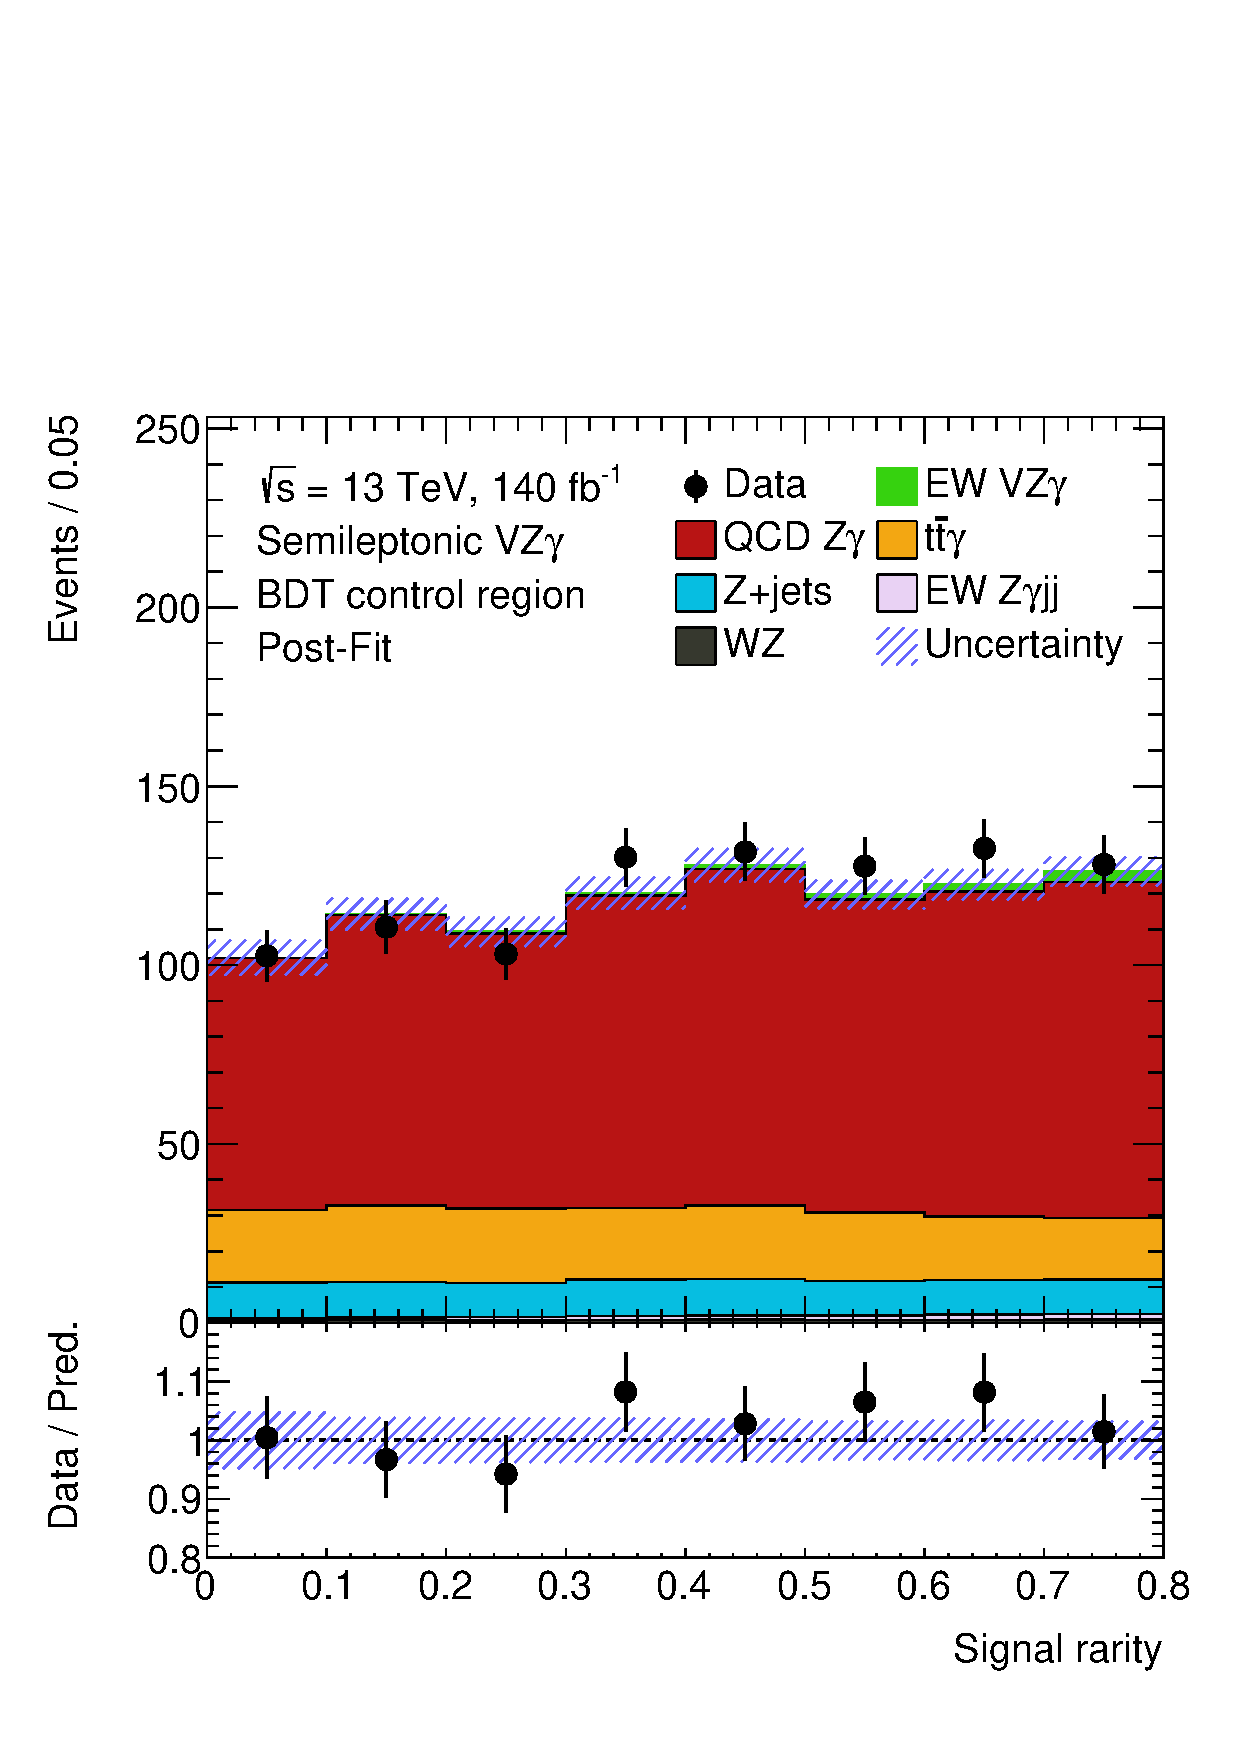
\includegraphics[width=\textwidth]{\resource{stack/CR_BDT_postFit.pdf}}
  \end{subfigure}
  \hfill
  \begin{subfigure}{.495\textwidth}
    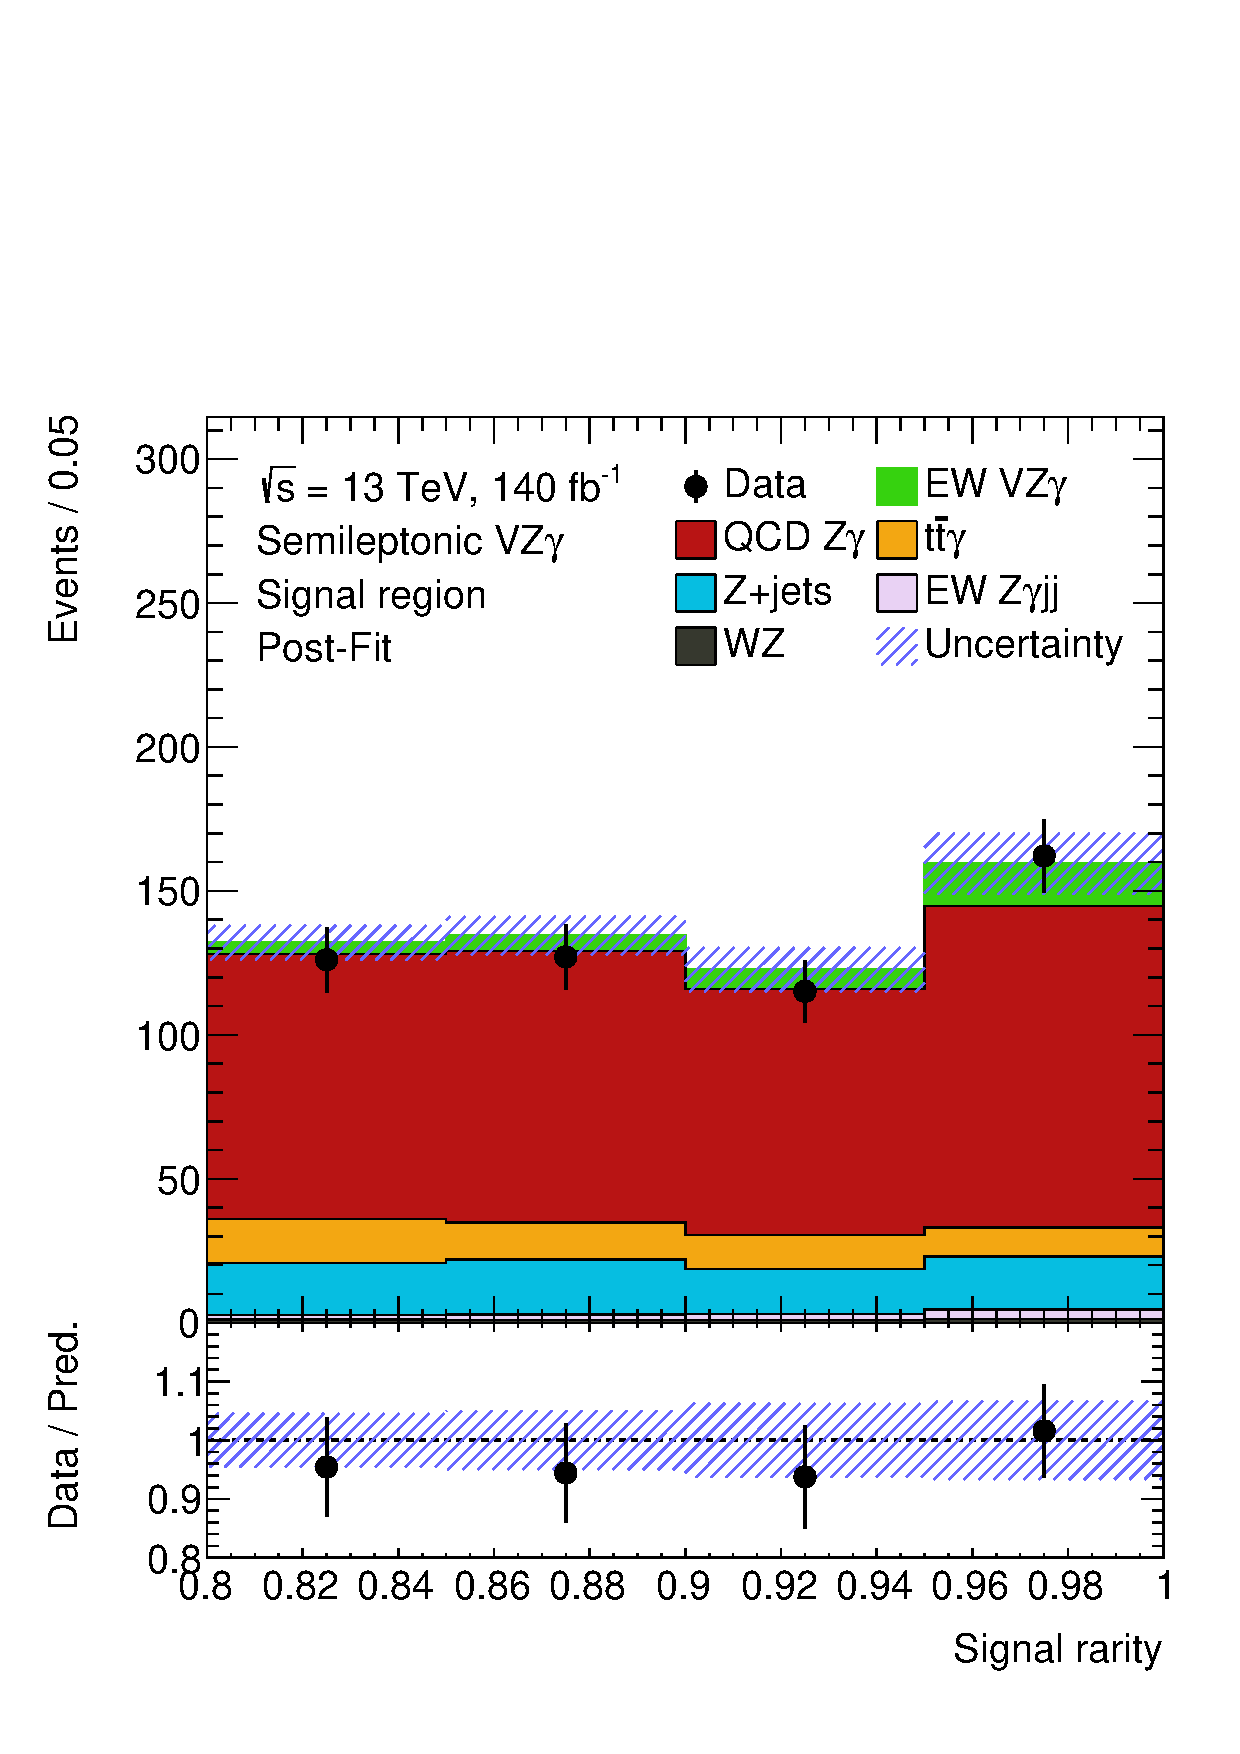
\includegraphics[width=\textwidth]{\resource{stack/SR_postFit.pdf}}
  \end{subfigure}
  \\[1em]%
  \begin{subfigure}{.495\textwidth}
    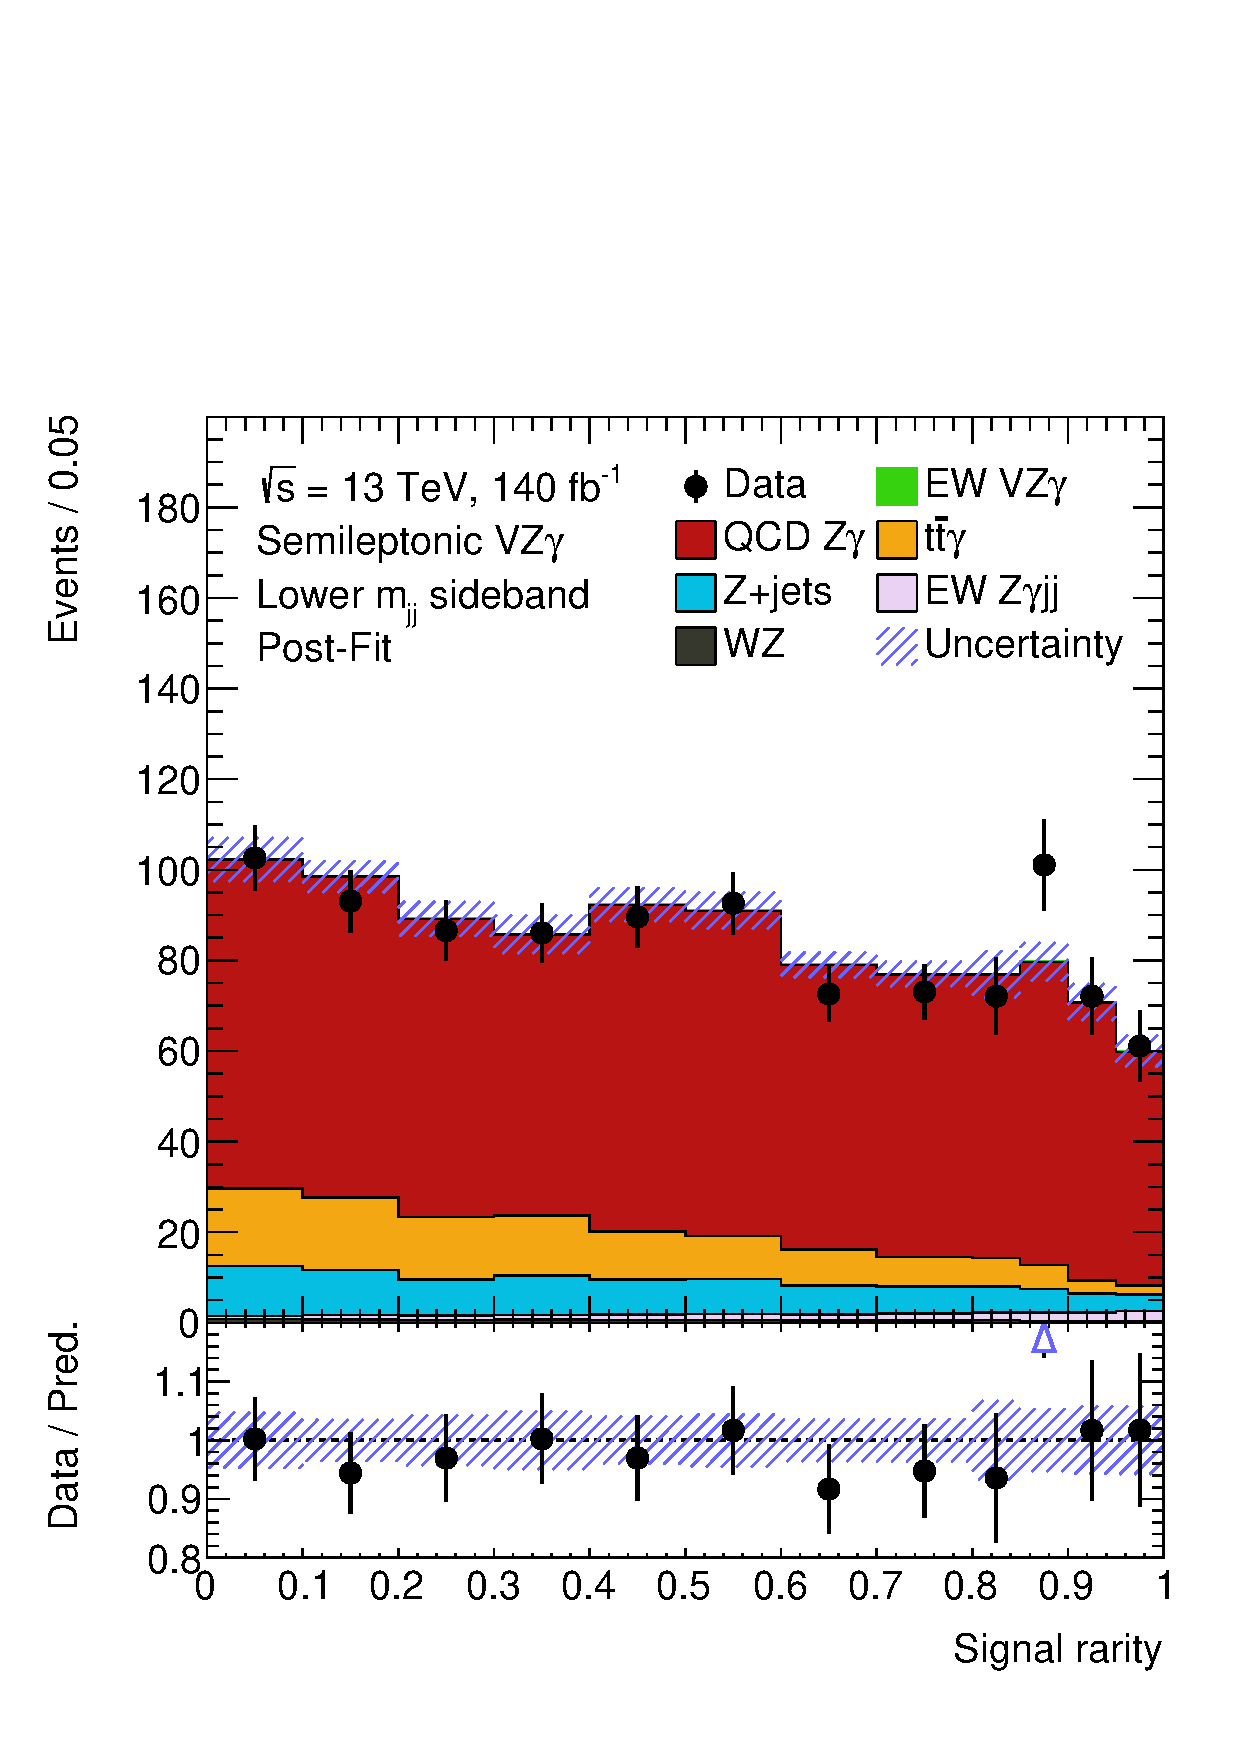
\includegraphics[width=\textwidth]{\resource{stack/CR_mjj_1_postFit.pdf}}
  \end{subfigure}
  \hfill
  \begin{subfigure}{.495\textwidth}
    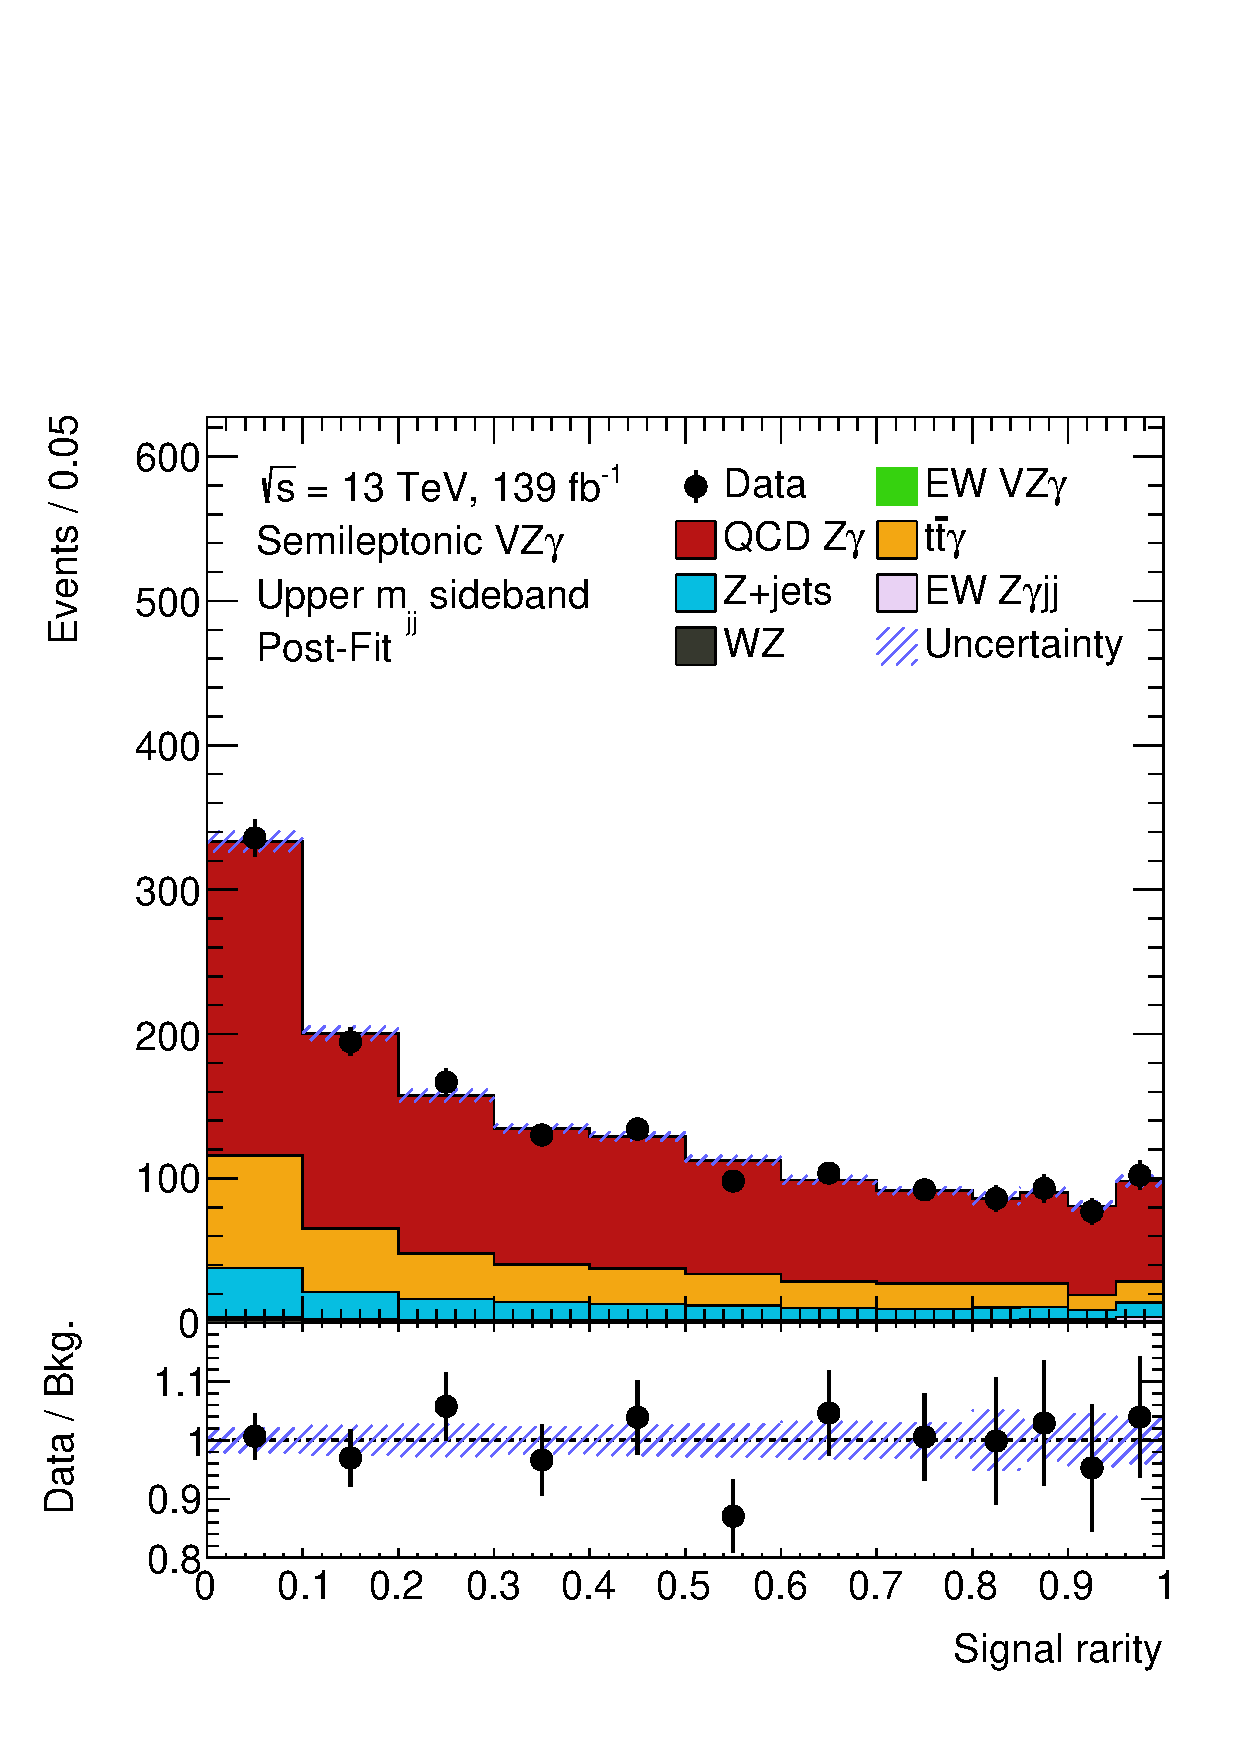
\includegraphics[width=\textwidth]{\resource{stack/CR_mjj_2_postFit.pdf}}
  \end{subfigure}
  \caption{
    Post-fit signal rarity distributions in each of the four regions used in the
    fit, as labelled. Uncertainty bands represent the combined uncertainties in
    each bin, with values constrained by the fit.
  }
  \label{fig:vzy-results-postfit}
\end{figure}

% Significance and limits
The observed significance of the signal process is 1.24 standard deviations,
from an expected significance of 1.40 standard deviations.
This does not meet the threshold to provide evidence on the existence of the
process. Instead a limit is set on the rate of production for signal events at
3.46 times the \ac{SM} expectation. This can be used to constrain any new
physics models that would enhance the cross-section for triboson \VZy
production.

%Injecting signal into the limit estimate: 1.000000
%Expected limit (median): 2.261164, worst case error: -0.026594
%Expected limit (-1 sig): 1.608560, worst case error: 0.028700
%Expected limit ( 1 sig): 3.203297, worst case error: -0.089267
%Expected limit (-2 sig): 1.188495, worst case error: 0.015355
%Expected limit ( 2 sig): 4.391544, worst case error: -0.135924
%Injected limit         : 3.044920, worst case error: 0.143740
%Observed limit         : 3.464933, worst case error: 0.234227
%Expected p-value mu = 1 (median)     : 0.186029, error: 0.000003
%Observed p-value (median)            : 0.107927, error: 0.000002
%Expected significance mu = 1 (median): 0.892623, error: -0.000011
%Observed significance (median)       : 1.237627, error: -0.000011

% Pulls and ranking (pulls necessary? don't understand them too well)
Statistical uncertainties make the largest contribution to the measurement, but
systematic uncertainties make a significant contribution. The largest systematic
contributions are shown in Figure \ref{fig:vzy-results-ranking}.
Pileup reweighting is the largest individual contribution, likely due to the
limited data statistics (see Section \ref{sec:vzy-projection}). Section
\ref{sec:methods-systematics} discusses the origin of pileup reweighting
uncertainties.
The second largest contribution is from jet flavour composition. This
uncertainty is reducible, as was done for the \ac{VBS} \Zy analysis, but there
was not sufficient time to implement it for this analysis. Several more of the
largest uncertainties are \ac{MC} statistics uncertainties in signal bins; these
are also reducible given large \ac{MC} samples. The effect of reducing some of
these systematic uncertainties is discussed in Section \ref{sec:vzy-projection}.

\begin{figure}[tbhp]
  \centering
  \includegraphics[width=.8\textwidth]{\resource{Ranking_mu_EWK.pdf}}
  \caption{
    Systematic uncertainties ranked by their post-fit impact on \muEW.
    Uncertainties labelled $\gamma$ represent \acs{MC} statistics uncertainties
    in the given bin.
  }
  \label{fig:vzy-results-ranking}
\end{figure}
% TODO more detail on what the ranking plot means
